% !TeX root = main.tex
\documentclass{sbrt}
\usepackage[english,brazil]{babel}
\usepackage[utf8]{inputenc}
\usepackage{amsmath}
\usepackage{natbib}
\usepackage{pgfplots}
\newtheorem{theorem}{Teorema}
\pgfplotsset{compat=1.18}

%% ---------------------------------------------

\begin{document}

\title{Autotune: como funciona a harmonização da voz humana}

\author{Carlos E. P. Silva, Gabriel M. Silvério, Geovanne B. Lopes, Matheus B. Frate}

\maketitle

%% ---------------------------------------------

\begin{resumo}
  O Autotune é um software que permite aos usuários alterar o tom de sua voz utilizando um algoritmo que analisa o sinal
  de áudio e, em seguida, ajusta o tom da voz para que ele esteja em harmonia com o tom desejado. Este artigo tem como
  objetivo explicar como funciona a harmonização da voz humana.
\end{resumo}
\begin{chave}
  Autotune, algoritmo, análise de sinal, equalização, filtragem, tom \hfill \break
\end{chave}

%% ---------------------------------------------

\begin{abstract}
  Autotune is a software that allows users to change the pitch of their voice using an algorithm that analyzes the audio
  signal and then adjusts the pitch of the voice to be in harmony with the desired pitch. The purpose of this article is
  to explain how voice harmony works.
\end{abstract}
\begin{keywords}
  Autotune, algorithm, signal analysis, equalization, filtering, pitch
\end{keywords}

%% ---------------------------------------------

\section{Introdução}

O auto-tune é um software que usa um algoritmo para processar sinais de voz humana. Ele analisa o sinal de áudio e, em
seguida, ajusta o tom da voz para que ele esteja em harmonia com o sinal. A ferramenta está extensivamente entrelaçada
na cena musical da atual geração de músicos~\cite{diaz2009fate}.

Há várias razões pelas quais os músicos podem optar por usar autotune para ajustar o tom de sua música.
Segundo~\cite{browning2014auto}, em primeiro lugar, o autotune pode ajudar a manter os instrumentos em sincronia, o que
é especialmente importante para os músicos que tocam em ensemble\footnote{Ensemble é um termo musical que se refere a um
grupo de instrumentos ou vozes que tocam ou cantam juntos.}. Em segundo lugar, o autotune pode ser usado para corrigir
erros de afinação, permitindo que os músicos toquem com mais precisão. Por fim, o autotune pode ser usado para criar
efeitos especiais de som, como vibrato e sustenido.

Este trabalho busca analisar especificamente o processo de harmonização da voz através de um algoritmo feito em Python,
o qual exemplificará e elucidará o tratamento necessário para harmonização do tom através dos dados obtidos.

%% ---------------------------------------------

\section{Fundamentação}

\subsection{Processamento de Sinais}

O primeiro passo para compreender o funcionamento do algoritmo é entender o que são sinais e como podem ser processados.
Conforme~\cite{prandoni2008signal}, em termos gerais, é o processo de analisar e manipular um sinal para extrair
informações úteis ou para alterar o sinal de alguma forma. Um sinal pode ser qualquer coisa, desde um som até um gráfico
de um fenômeno físico. O processamento de sinais pode ser feito de forma analógica utilizando circuitos eletrônicos ou
digital utilizando algoritmos e computadores.

\subsection{Notas Musicais}

Segundo~\cite{moretti2003prototipo}, notas musicais são os sons emitidos por instrumentos musicais ou vozes que, em
conjunto, formam uma melodia ou uma composição. As notas musicais são classificadas por sua altura (tom) ou frequência.
A frequência é a medida da velocidade de vibração de um som e é medida em hertz (Hz). Quanto maior a frequência, mais
agudo é o som. A Figura 1 representa dois sinais de diferentes frequências. O sinal representado pelo traço mais cheio
tem a metade da frequência do outro.


\begin{figure}[ht]
  \centering
  \begin{tikzpicture}
    \begin{axis}[ xlabel=Tempo, ylabel=Amplitude, xlabel style={anchor=west, at={(axis description cs:1,0)}}, ylabel
    style={anchor=south, at={(axis description cs:0.15,1)}, rotate=-90}, width=.5\textwidth, height=6cm, domain=-0:2*pi,
    samples=50, smooth, ymin=-1, ymax=1, axis lines=left, axis line style={->}, xtick=\empty, ytick=\empty, grid=none, x
    tick label style = {black}, enlargelimits={abs=0.2} ] \addplot[mark=none]{sin(deg(2*pi*x))}; \addplot[mark=none,
    style={line width=1.5pt}]{sin(deg(pi*x))};
    \end{axis}
  \end{tikzpicture}
  \caption{\label{fig:sine}Diferentes frequências.}
\end{figure}

Conforme~\cite{moretti2003prototipo} elucida, a notação musical define sete notas naturais: Dó, Ré, Mi, Fá, Sol, Lá e Si
(C, D, E, F, G, A, B). Elas são denominadas notas naturais, pois formam a base de todas as escalas e harmonia musical.
Por sua vez oitava é o espaço entre a primeira nota de uma escala e a oitava nota, e é considerada a maior unidade de
som musical.

\begin{quote}
  ``Oitava é o espaço musical que compreende duas notas de mesmo nome, mas de alturas diferentes. Por exemplo, uma
  oitava é o espaço entre uma nota dó a próxima nota dó na escala, mais aguda que a
  primeira''~\cite{moretti2003prototipo}.
\end{quote}

Semitons, por sua vez, são os intervalos entre as notas naturais. A escala cromática é uma escala que contém todas as
notas naturais, e também todos os semitons, totalizando doze notas. A tabela~\ref{tab:freq} mostra a relação entre a
frequência e a altura do som.

\begin{table}[ht]
  \centering
  \caption{\label{tab:freq} Frequência e altura do som.}
  \vspace{-0.2cm}
  \begin{tabular}{c c c c c c}
       & \multicolumn{4}{c}{Frequência em Hz}                                                 \\
    Nº & Nota Musical                         & 2ª Oitava & 3ª Oitava & 4ª Oitava & 5ª Oitava \\
    \hline
    1  & C                                    & 65.41     & 130.81    & 261.63    & 523.25    \\
    2  & C\#                                  & 69.30     & 138.59    & 277.18    & 554.37    \\
    3  & D                                    & 73.42     & 146.83    & 293.66    & 587.33    \\
    4  & D\#                                  & 77.78     & 155.56    & 311.13    & 622.25    \\
    5  & E                                    & 82.41     & 164.81    & 329.63    & 659.26    \\
    6  & F                                    & 87.31     & 174.61    & 349.23    & 698.46    \\
    7  & F\#                                  & 92.50     & 185.00    & 369.99    & 739.99    \\
    8  & G                                    & 98.00     & 196.00    & 392.00    & 783.99    \\
    9  & G\#                                  & 103.83    & 207.65    & 415.30    & 830.61    \\
    10 & A                                    & 110.00    & 220.00    & 440.00    & 880.00    \\
    11 & A\#                                  & 116.54    & 233.08    & 466.16    & 932.33    \\
    12 & B                                    & 123.47    & 246.94    & 493.88    & 987.77    \\
  \end{tabular}
\end{table}

\subsection{Transformada de Fourier}

Segundo~\cite{richardson1978fundamentals}, o método define-se como um procedimento matemático que transforma um sinal de
domínio temporal em funções de domínio de frequência complexas. Ela foi desenvolvida por Jean-Baptiste-Joseph Fourier,
um matemático francês que descobriu que qualquer sinal periódico pode ser expressado como uma soma de sinais senoidais
de diferentes frequências e amplitude.

Conforme~\cite{richardson1978fundamentals} distingue, existem dois tipos de Transformada de Fourier: a Contínua e a
Discreta. A Transformada de Fourier Contínua ou Continuous Fourier Transform (CFT) é utilizada para transformar sinais
de tempo contínuos em sinais de frequência contínua. Por sua vez, a Transformada de Fourier Discreta ou Discrete
Fourirer Transform (DFT) é utilizada para sinais de tempo discretos em sinais de frequência discreta. Neste trabalho
será definido a Transformada de Fourier Discreta, pois os sinais utilizados são discretos.

A Transformada de Fourier Discreta de um vetor $x_m$ de tamanho $N$ de um sinal contíguo $x(t)$ no domínio do tempo é
uma representação complexa de tamanho $N$ do vetor $x_m$ no domínio da frequência. A representação é definida por:

\begin{equation} \label{eq:fourier}
  {X_k} = \sum_{n=0}^{N-1} x_n W^{kn}, k = 0, 1, \dots, N-1 \\
\end{equation}

Onde W é a raiz da unidade primitiva de tamanho N, $e^{-j \frac{2\pi}{N}}$ e j é a unidade imaginária, $\sqrt{-1}$. A
Transformada de Fourier Inversa, por sua vez, é uma representação do vetor $X_k$ no domínio do tempo. A representação é
dada por:

\begin{equation} \label{eq:fourier_inv}
  x_l = \frac{1}{N} \sum_{k=0}^{N-1} {X_k} W^{-kl}, l = 0, 1, \dots, N-1
\end{equation}

\subsection{Transformada Rápida de Fourier}

A Transformada Rápida de Fourier (FFT), é um metodo que  converte um sinal em componentes espectrais individuais para
fornecer a frequência do sinal.

Desenvolvido em 1965 por  J. W. Cooley (IBM) e J. W. Tukey (Bell Labs), teve como objetivo principal otimizar a
utilização da do DFT, para que fosse executada de forma mais rápida e com um trabalho computacional
reduzido~\cite{martins2016analise}.

Enquanto a implementação do DTF possuiam um custo computacional de $O(N^2)$ com a implementação do FFT o custo foi
reduzido para $O(N \log_2{N})$. A FFT mudou o uso de polinômios trigonométricos interpolatórios, organizando de forma
que o número de pontos usados pode ser fatorado em potências de dois, dessa forma, sua utilização é mais eficiente por
ser mais rápida e por realizar o cálculo da DFT e também sua inversa~\cite{reis2008implementaccao}.

\subsection{Autocorrelação}

A função de autocorrelação é utilizada para determinar a frequência fundamental de um sinal e é definida
por~\cite{fong2016adaptive}:

\begin{equation}
  \begin{gathered}
    R(\tau) = \frac{1}{N - \tau} \sum_{m=0}^{W - 1 - \tau} x_m x_{m + \tau} \\
    \tau = 0, 1, \dots, N - 1
  \end{gathered}
\end{equation}

Onde $\tau$ é o deslocamento entre os pontos de amostragem, $x_m$ é o sinal de entrada e $N$ é o tamanho da janela de
amostragem.

\subsection{Janelamento}

O janelamento é uma técnica usada na análise de sinais, comumente aplicada em processos de filtragem e transformações.
Ele consiste em dividir o sinal original em diversas partes ou janelas, cada qual contendo um número específico de
amostras do sinal. A principal vantagem desta abordagem está na possibilidade de analisar/manipular os dados contidos
nas janelas individualmente, sem que haja interferências das outras partes do sinal e minimzando o efeito de leakage
causado pela amostragem da FFT~\cite{deimplementaccao}.

Abordaremos especicamente o método de janelamento TD-PSOLA, do inglês, Time Domain Pitch Synchronous Overlap and Add ou
Sobreposição e Adição Sincronizadas em relação ao Tom no Domínio do Tempo. Enquanto o janelamento tradicional é feito no
domínio da frequência, o TD-PSOLA é feito no domínio do tempo e é baseado em overlap-add que consiste em selecionar uma
janela de áudio contendo um período vocal específico, analisá-lo para extrair as informações necessárias sobre o pitch e
então realizar os cálculos necessários para modificar a taxa de amostragem sem distorcer as formantes vocais. A partir
disso, essa janela editada é adicionada à próxima janela não processada até completar todo o arquivo
áudio~\cite{cheng2012design}.

%% ---------------------------------------------

\section{Desenvolvimento}

PyAutoTune é uma biblioteca para Python que usa um algoritmo desenvolvido por Tom Baran denominado
Autotalent~\cite{baran2011autotalent}. O algoritmo é capaz de analisar o som de uma voz humana e identificar as notas
musicais que estão sendo cantadas. Em seguida, pode-se ajustar a voz para que esteja sempre dentro da escala musical
definida pelo usuário.

Além disso, a biblioteca também permite que o usuário ajuste o timbre da voz, adicionando efeitos como vibrato
artificial ou alterando as formantes. Autotalent foi criado para processar melodias musicais, sejam elas cantadas por
voz ou tocadas em algum tipo de instrumento.

\subsection{Funcionamento}

O script consiste principalmente num detector de tom e num transpositor de tom. O detector detecta o tom do sinal
sonoro, e, de acordo com este valor e os valores dos controles, o transpositor altera o tom para uma frequência maior ou
menor, resultando em um sinal de saída que está em harmonia.

Tanto o detector de tom quanto o afinador de tom são projetados para operar em sinais monofônicos. Dito isso, para
alcançar a harmonia vocal em um sinal de mais de um canal, deve-se processar cada uma das partes monofônicas
separadamente.

O detector de tom encontra o período do som através do autocorrelação, e o transpositor usa a técnica de sobreposição e
adição de sinais sincronizada com o período do som de entrada.

A autocorrelação é calculada pelo produto do sinal com ele mesmo, deslocado por um determinado número de amostras. O
resultado da autocorrelação é uma função que indica a similaridade entre o sinal e seu atraso. A FFT é utilizada para
calcular a autocorrelação de forma mais eficiente, reduzindo o tempo necessário para processar os dados. Isto é, a FFT é
utilizada para calcular a autocorrelação do sinal sonoro, que indicará o período do som~\cite{myint2010spatial}.

O sinal transpositado é uma sobreposição e adição dos harmônicos fundamentais do sinal original, onde cada um está
deslocado em frequência pelo valor da taxa de alteração escolhida. Esses novos harmônicos são então todos os mesmos
períodos que o fundamental original, resultando num tom mais alto (ou mais baixo), dependendo da direção da
transposiçao~\cite{laprie1998automatic}.

\begin{quote}
  ``Por exemplo, se a frequência da voz estiver em 435 Hz a voz está desafinada, pois não existe um tom nessa
  frequência, então ajusta-se para o tom mais próximo, que é Lá de 440 H''~\cite{deimplementaccao}.
\end{quote}

\subsection{Parâmetros}

\begin{itemize}
  \item CONCERT\_A: Frequência do tom A4 (440 Hz) utilizada como referência para o afinamento.
  \item CORR\_SMOOTH: O quão abrupto a correção de tom deve ser.
  \item CORR\_STR: Fator de correção de tom.
  \item FIXED\_PITCH: O tom para o qual o sinal de entrada deve ser transposto.
  \item FIXED\_PULL: Fator de afinação do tom para o tom fixo.
  \item FORM\_CORR: Habilita a correção formante.
  \item FORM\_WARP: Fator de correção de formante.
  \item LFO\_DEPTH: Fator de profundidade do LFO (Low Frequency Oscillator).
  \item LFO\_QUANT: Habilita a quantização do LFO.
  \item LFO\_RATE: Taxa de variação do LFO em Hz.
  \item LFO\_SHAPE: Forma do LFO. -1 = quadrada, 0 = senoidal, 1 = triangular.
  \item LFO\_SYMM: Simetria do LFO.
  \item MIX: Fator de mistura do sinal original com o sinal transpositado.
  \item PITCH\_SHIFT: O número de notas em escala para o qual o sinal transposto é deslocado.
  \item SCALE\_ROTATE: Número de notas em escala pelo qual a escala de saída é rotacionada na conversão de volta para
  semitons a partir de notas de escala.
\end{itemize}

\subsection{Utilização}

A biblioteca pode ser utilizada de duas formas: como um script ou como uma biblioteca. Para utilizá-la como um script,
basta executar o arquivo \textit{setup.py} com o Python 3 e utilizar o script de exemplo fornecido. Para utilizá-la como
uma biblioteca, basta instalar o arquivo \textit{setup.py} e instanciar a classe \textit{AutoTune}.

\subsection{Resultados}

A biblioteca foi testada com o script e áudio de exemplo fornecido pelo autor. O áudio de entrada é uma gravação de uma
voz humana alternando entre alturas de tom. O áudio de saída é o áudio de entrada com o tom ajustado para que fique com
o tom mais próximo do tom A4 (440 Hz). O áudio de entrada e saída podem ser ouvidos na Figura~\ref{fig:resultado}.

\begin{figure}[h]
  \centering
  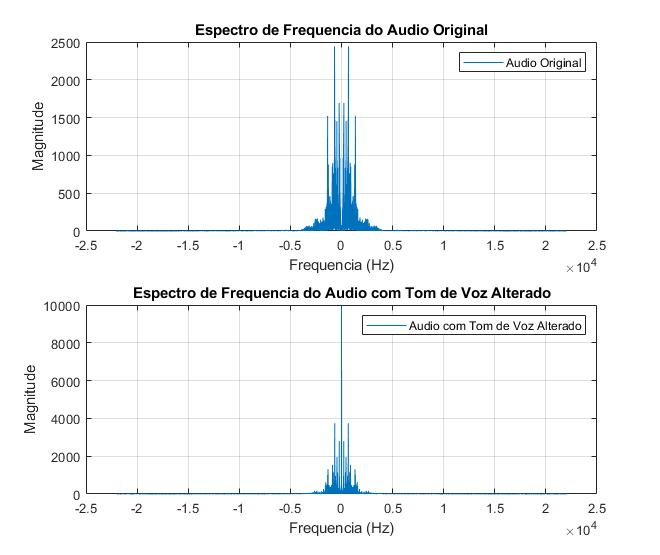
\includegraphics[width=0.5\textwidth]{resultado.jpg}
  \caption{Áudio de entrada e saída}
  \label{fig:resultado}
\end{figure}

%% ---------------------------------------------

\section{Conclusões}

Em linhas gerais, é possível ver que ao calcular a autocorrelação utilizando a FFT podemos obter o período do som, e a
partir dele podemos sobrepor e adicionar os harmônicos fundamentais do sinal original para que seja feita a alteração no
tom, seja para um tom mais alto ou mais baixo. Com o resultado nós podemos analisar e visualizar a mudança da frequência
do som processado.

A biblioteca utilizada nos permite realizar essas alterações e criar um arquivo de áudio novo para que seja feita as
comparações com o áudio original e ver as correções que foram feitas. 

Os gráficos obtidos através da leitura das frequências do áudio original e do áudio alterado no software matlab
confirmam a alteração da frequência. É possível observar que a frequência no áudio alterado está maior, pois sofreu a
alteração do script para alcançar um tom mais agudo, condizendo com o resultado que era esperado. 

%% ---------------------------------------------

\bibliographystyle{unsrt}
\bibliography{refs}

%% ---------------------------------------------

\end{document}
